%%%%%%%%%%%%%%%%%%%%%%%%%%%%%%%%%%%%%%%%%%%%%%%%%%%%%%%%%%%%%%%%%
% Contents : The home chapter
% $Id : grisbi-manuel-home.tex, v 0.4 2002/10/27 Daniel Cartron
% $Id : grisbi-manuel-home.tex, v 0.5.0 2004/06/01 Loic Breilloux
% $Id : grisbi-manuel-home.tex, v 0.6.0 2011/11/17 Jean-Luc Duflot
% some of its content was in menus chapter :
% $Id: grisbi-manuel-menus.tex, v 0.5.0 2004/06/01 Loic Breilloux
% $Id : grisbi-manuel-home.tex, v 0.8.9 2012/04/27 Jean-Luc Duflot
% $Id : grisbi-manuel-home.tex, v 1.0 2014/02/12 Jean-Luc Duflot
%%%%%%%%%%%%%%%%%%%%%%%%%%%%%%%%%%%%%%%%%%%%%%%%%%%%%%%%%%%%%%%%%

\chapter{Front page\label{home}}


When the application starts, Grisbi displays this
\ifIllustration Front pagel\refimage{home-img} page.
\else d'accueil.
\fi
This is the start page of the program; it can be accessed at any time by clicking on the  \menu{Accounts} tab. 

You can view the Grisbi window in full screen display \indexword{full screen mode}\index{affichage !plein écran}\index{plein écran !affichage} using the function key \key{F11}, and toggle between full screen and normal mode with the same key.

\ifIllustration
% image centrée
\begin{figure}[htbp]
\begin{center}
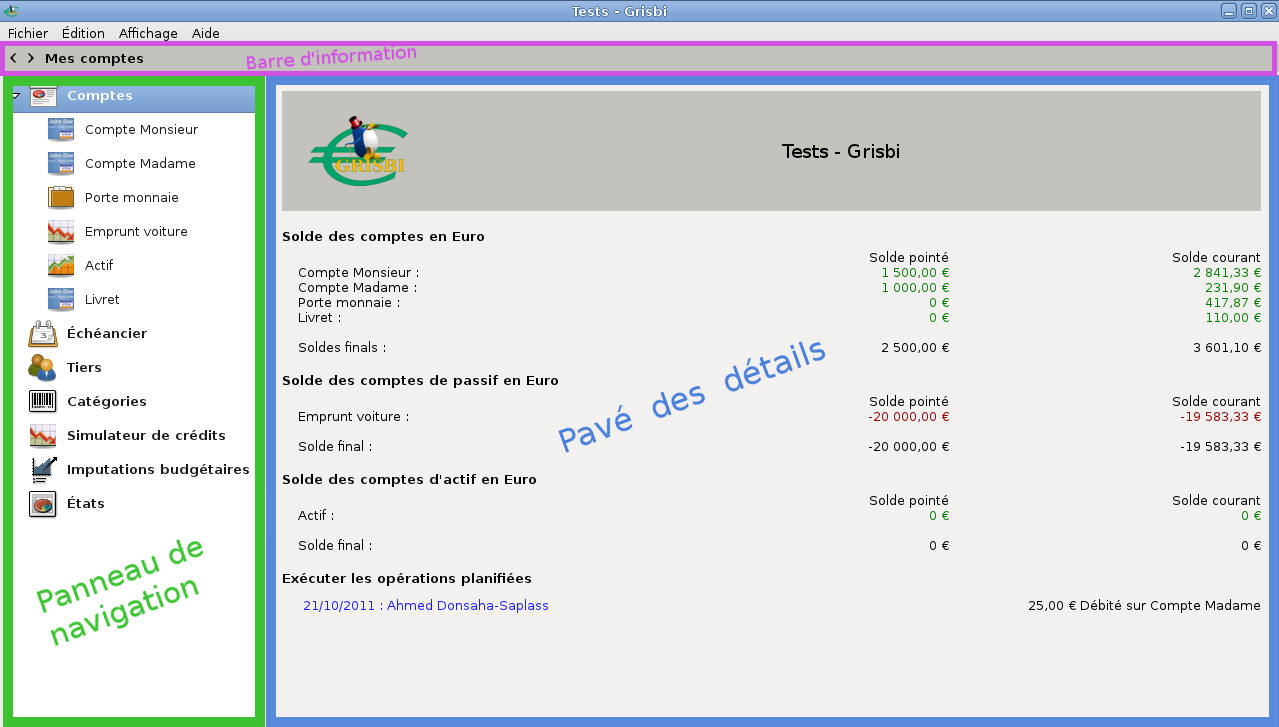
\includegraphics[scale=0.35]{image/screenshot/home}
\end{center}
\caption{Page d'accueil}
\label{home-img}
\end{figure}
% image centrée
\fi

All Grisbi screens have the same general appearance. It displays a menu bar that gives access to most of Grisbi's important features, and three main areas:

\begin{itemize}
	 \item the information bar, under the menu bar;
	 \item the navigation panel;
	 \item the main screen area.
\end{itemize}

\ifIllustration 
These three zones, specific to Grisbi, are outlined in different colors in the figure to identify them \refimage{home-img}.
\else
\fi

\section{Information bar\label{home-synthesis}}

The information bar displays the name of the current tab displayed, and can display, to the far right, certain balances related to what is selected in the main screen area.

% espace pour changement de thème
\vspacepdf{5mm}

To select one of the tabs displayed in the navigation panel click one or more times on one of the two small triangles on the top left of the panel.  The items displayed are : \menu{Accounts}, \menu{Scheduler}, \menu{Payees}, \menu{Credits simulator}, \menu{Categories}, \menu{Budgetary lines} and \menu{Reports}.  If the \menu{Accounts} and \menu{Reports} items have been expanded to display their sub categories these will also be displayed one by one.

% Pas de commande au clavier pour cette fonction
\textbf{Note} : These triangle symbols can be replaced, depending on the theme of the desktop environment or window manager you are using, by other characters such as +, -,>, <, and so on.

% espace pour changement de thème
\vspacepdf{5mm}
The content of the selection is displayed in the details box.

% espace pour changement de thème
\vspacepdf{5mm}
These features can be used instead of clicking directly in the navigation panel when its width is reduced to zero and you can not access it directly.


\section{Navigation panel\label{home-accounting}}

The navigation pane displays in bold the list of tabs:  \menu{Accounts}, \menu{Scheduler}, \menu{Payees}, \menu{Credits simulator}, \menu{Categories}, \menu{Budgetary lines} et \menu{Reports}. By clicking on the small black triangle to the left of the  \menu{Accounts} or \menu{Reports} tabs,  you can scroll or roll up the list of their sub-tabs. You can change the order of tabs and sub-tabs by clicking on one of them and moving it up or down the list.

\textbf{Note} : These triangles can be replaced, depending on the theme of the desktop environment or window manager you are using, by other characters such as +, -,>, <, and so on.

% espace pour changement de thème
\vspacepdf{5mm}

You can select one of these tabs or sub-tabs by clicking on its name. You can also move the selection in this list of tabs and sub-tabs with the \key{Up Arrow}, \key{Down Arrow}, \key{Page Up} ou \key{Page Down} keys, or with the mouse wheel. 

% espace pour changement de thème
\vspacepdf{5mm}
The content of the selection is displayed in the details box.

% espace pour changement de thème
\vspacepdf{5mm}
You can reduce or enlarge the width of the navigation panel by clicking on the thin vertical bar between this panel and the detail pad, and moving it. If the width of the panel has been reduced to zero, or enlarged to the maximum of the width of the Grisbi window, it is necessary to find this bar, it may be to the left or to the right of the window, and to slide it to the desired place.

% espace pour changement de thème
\vspacepdf{5mm}

The \indexword{menus contextuels}\index{menu contextuel}, shortcut context menu menus, accessible by a right-click of the mouse, are available on the elements of this panel and offer the following functions::

\begin{itemize}
	 \item sur \menu{Accounts} :
		\begin{itemize}
			 \item \menu{New account} ;
		\end{itemize}
	 \item On any account : 
		\begin{itemize}
			 \item \menu{New account},
			 \item \menu{Delete this account} ;
		\end{itemize}
	 \item sur \menu{Payees} :
		\begin{itemize}
			 \item \menu{New payee},
			 \item \menu{Delete selected payee},
			 \item \menu{Edit selected payee},
			 \item \menu{Manage payees},
			 \item \menu{Remove unused payees} ;
		\end{itemize}
	 \item sur \menu{Categories} : 
		\begin{itemize}
			 \item \menu{New category},
			 \item \menu{Delete selected category},
			 \item \menu{Edit the selected category},
			 \item \menu{Import a file of categories (.csgb)},
			 \item \menu{Export a file of categories (.csgb)} ;
		\end{itemize}
	 \item sur \menu{Budgetary lines} :
		\begin{itemize}
			 \item \menu{New budgetary line},
			 \item \menu{Delete selected budgetary line},
			 \item \menu{Edit selected budgetary line},
			 \item \menu{Import a file of budgetary lines (.isgb)},
			 \item \menu{Export a file of budgetary lines (.isgb)} ;
		\end{itemize}
	 \item sur \menu{Report} : \menu{New report} ;
	 \item On any report : 
		\begin{itemize}
			 \item \menu{New report},
			 \item \menu{Delete this report}.
		\end{itemize}
\end{itemize}

\ifIllustration
\else
% saut de page pour titre solidaire
\newpage
\fi


\section{Details window\label{home-details}}

The Details window displays all the details on the tabs or sub-tab selected by the Information Bar or Navigation Panel. This is the main work area of Grisbi.
You can reduce or enlarge its width by clicking on the thin vertical bar between this tile and the navigation panel, and dragging it. If the width of the this area has been reduced to zero or enlarged to the maximum of the width of the Grisbi window, you must find this bar, it will be to the right or left of the window, and drag it to the desired position.
 
\subsection{View home page\label{home-details-homepage}}

To view the home page, select the Accounts tab; then the details block shows, from top to bottom:

\begin{itemize}
	 \item in a box on a gray background, the \menu{Grisbi} icon on the left and on the right \indexword{titre}\index{affichage !titre}\index{titre !page d'accueil} the title of the accounts file you currently have loaded, in the form  \og labelled - Grisbi\fg{} ; you can define this name in one of three ways the \menu{Edit preferences} menu (see the paragraph \vref{setup-display-addresses-titles}, \menu{??Titres??}) ; this can be useful if you manage multiple accounting entities:
		\begin{itemize}
			 \item The \menu{Accounting Entity} : This is the name you use to identify the type of account e.g. \og My Accounts \fg{} or \og Business\fg{}, which you entered when the account file was created; you can edit it here in the   \menu{Account Name field} ; this can be useful if you manage multiple accounting entities, \indexword{entités comptables}\index{entité comptable}, 
			 \item The \menu{Account holder} :the name of the owner (or ??manager??) of the last account accessed; if the holder is not defined in the account properties, Grisbi displays the name of this account,
			 \item le \menu{Accounts file name} :  This is the name of the file in the current directory, in the form  \file{nom\_de\_\_votre\_fichier.gsb}, and this is the default choice;
		\end{itemize}
		
	 \item for each currency separately, for all accounts and \indexword{groupes de comptes}\index{groupe de comptes},  under the label \menu{Close Balance} et \menu{Current Balance} :
		\begin{itemize}
			 \item the balance of the bank and cash accounts, the partial balance of the groups of accounts and their final balance,
% saut de ligne pour indentation correcte de la note dans la liste

			 \textbf{Note} : you can adjust the display order of the partial balances of the account groups (see the section \vref{setup-general-home-partBalance}, \menu{Partial balances of the list of accounts}).			 
			 \item the balance of the liability accounts and their final balance,
			 \item the balance of the asset accounts and their final balance;
		\end{itemize}
	\item the \indexword{alertes des opérations planifiées}\index{alerte !opération planifiée} with their date, wording and amount, according to the choices made in the \menu{Edit - Preferences menu} (voir la section \vref{setup-general-planned}, \menu{Timeline}) ;
	\item the list of accounts whose balance has fallen below the minimum authorized balance \menu{minimum authorized balance} ;
	\item the list of accounts whose balance has fallen below the  \menu{required Minimum Balance}.
\end{itemize}

% espace avant Attention ou Note  : 5 mm
\vspacepdf{5mm}

5mm

\textbf{Note} : For definitions of \menu{Minimum Allowable Balance} and \menu{Desired  minimum balance}, see the \vref{accounts-properties}, \menu{Account Properties} section.

% espace pour changement de thème
\vspacepdf{5mm}

The account labels are displayed in black; as the mouse moves over any of the entries, this color changes to gray.
A balance greater than the desired Minimum Balance is displayed in dark green; as the pointer passes on its line, this color changes to light green.

The account labels are displayed in black{\couleur} ; as the mouse moves over the line of one of them, this color changes to gray {\couleur}.
A balance greater than the  \menu{desired Minimum Balance}  is displayed in dark green {\couleur} ; as the pointer passes on its line, this color changes to light green {\couleur}.



A balance less than the \menu{Minimum Balance Required} and greater than the \menu{Minimum Balance authorized} is displayed in orange{\couleur} ; as the pointer passes on its line, this color changes to light orange{\couleur}.
A balance less than the  \menu{Minimum Authorized Balance}  is displayed in red{\couleur} ; as the pointer passes over its line, this color changes to light red{\couleur}.

When you move the mouse pointer over the line of an account, any color change indicates that if you click (right or left) with the mouse, the records contained in the highlighted account is displayed, as if it had been selected with the information bar or navigation panel.

A partial balance, which is a group of accounts, is displayed in black{\couleur}.If it is negative, it may appear in dark red{\couleur}, but only if it has been configured as well (see  \vref{setup-general-home-partBalance}, \menu{Soldes partiels de la liste des comptes}). A partial balance line does not change color when the mouse pointer is over it, because you can not view the operations of an account group.


%itemize - kept until \menu operation
%Font fonts, logo logo and color colors: setup-display-logo section;
%Titles: section setup-display-addresses-titles;
%Calculation of balances: paragraph setup-general-home-balance;
%Partial balances in the list of accounts: paragraph setup-general-home-partBalance;
%Schedule Alerts: setup-general-planned section;
%accounts under the Minimum authorized balance minimum balance allowed: accounts-properties section;
%accounts under the minimum balance wanted minimum balance wanted: accounts-properties section.
%itemize
% setup-general-home-final, plural of final!


% espace pour changement de thème
\vspacepdf{5mm}
You can configure certain aspects of the display of this home page in the \menu{Édition - Préférences} or in the \menu{Propriétés} tab of each account :
\begin{itemize}
	 \item \menu{\indexword{Polices}\index{polices}, \indexword{logo}\index{logo} et \indexword{couleurs}\index{couleurs}} : section \vref{setup-display-logo} ;
	 \item \menu{Titres} : section \vref{setup-display-addresses-titles} ;
	 \item \menu{Calcul des soldes} : paragraphe \vref{setup-general-home-balance} ;
	 \item \menu{Soldes partiels de la liste des comptes} : paragraphe \vref{setup-general-home-partBalance} ;
	 \item \menu{Alertes de l'échéancier} : section \vref{setup-general-planned} ;
	 \item comptes sous le \menu{\indexword{Solde minimal autorisé}}\index{solde !minimal autorisé} : section \vref{accounts-properties} ;
	 \item comptes sous le \menu{\indexword{Solde minimal voulu}}\index{solde !minimal voulu} : section  \vref{accounts-properties}.
\end{itemize}

In particular, if you find a spelling error in this page, you can correct it: see the paragraph \vref{setup-general-home-final}, \menu{Pluriel de final} !

\ifIllustration
% saut de page pour paragraphe solidaire
\newpage
\fi

\section{menu bar\label{home-menus}}

As in many graphics applications, most of Grisbi's important features are accessible through the menus in the \indexword{barre de menus}\index{barre de menus}. The features are detailed below.


\subsection{Menu \menu{Fichier}\label{home-menus-file}}

This menu includes the following functions :


%New account file: 
%Open: 
%Latest files:
%Save: 
%Save As: 
%Import a file: 
%Export to QIF / CSV file: 
%Create an archive: 
%Export an archive to a GSB / QIF / CSV file: 
%Debug the account file: 
%Make the account file anonymous: 
%Make the QIF file anonymous: 
%Debug mode: 
%Close: 
%Leave: Grisbi farm; 

\begin{itemize}
	\item \menu{Nouveau fichier de comptes} : creates a new account file; the current file is closed and a new empty file is created with an empty account (shortcut key \key{Ctrl}\key{N}),  see the \vref{start-newfile} section ; not to be confused with the creation of a new account;
	\item \menu{Ouvrir} : open an accounts file  (shortcut key  \key{Ctrl}\key{O}) ;
	\item \menu{Derniers fichiers} : displays the list of the last n files opened with Grisbi (only if there have been several); this number is configurable in the \menu{Edition - Préférences}, see the \vref{setup-general-files-manage}, \menu{Gestion des fichiers de compte} section ;
	\item \menu{Enregistrer} : Saves the current account file  (shortcut key \key{Ctrl}\key{S}) ;
	\item \menu{Enregistrer sous} : opens a file manager to save the current accounts file with the name and location of your choice; Grisbi defaults to the current directory, the name of the current accounts file, with the \file{.gsb} extension ;
	\item \menu{Importer un fichier} :starts the file import wizard of another software; see  \vref{move-import-importinit} ;
	\item \menu{Exporter vers un fichier QIF/CSV} :starts the Export Account File Wizard; see \vref{move-export} ;	
	\item \menu{Créer une archive} : starts the archive creation wizard; see \vref{datamanagement-history-new} ;	
	\item \menu{Exporter une archive vers un fichier GSB/QIF/CSV} : starts the archive export wizard; see \vref{datamanagement-history-export} ;
	\item \menu{Déboguer le fichier de compte} :Starts the debug wizard for this file, which will help you look for inconsistencies in your account file; see  \vref{maintenance-file-debug} ;
	\item \menu{Rendre anonyme le fichier de comptes} :starts the wizard that produces an anonymous copy of your account file; this file can be attached to a bug report; see \vref{maintenance-file-anonymous} ;	
	\item \menu{Rendre anonyme le fichier QIF} :  starts the wizard that produces an anonymous copy of this file; this file can be attached to a bug report; see \vref{maintenance-QIF-anonymous} ;	
	\item \menu{Mode de débogage} : puts Grisbi in debug mode, which creates a log file of events; see \vref{maintenance-debug-mode} ; 	
	\item \menu{Fermer} : closes the current accounts file; Grisbi offers to save it if you have not already done it (keyboard shortcut \key{Ctrl}\key{W}) ;
	\item \menu{Quitter} : ferme Grisbi ; Grisbi prompts you to save the account file if you have made any changes (raccourci-clavier \key{Ctrl}\key{Q}).
\end{itemize}


\subsection{Menu \menu{Édition}\label{home-menus-edit}}

Ce menu comprend les fonctions suivantes :

%itemize
%Edit operation: see transactions-modify section, Editing an operation;
%New operation: see transactions-new section, Entering a new transaction;
%Delete an operation: see transactions-delete section, Deleting an operation;
%Use the selected operation as a template: see transactions-model section, Operation selected as template;
%Clone the operation: see transactions-duplicate section, Cloning an operation;
%Convert to scheduled operation: see the transactions-schedule section, Converting an operation to a planned operation;
%Move the operation to another account: see the transactions-move section, Moving an operation to another account;
%New account: see accounts-new section, Creating a new account;
%Delete the current account: see the accounts-delete section, Deleting an account;
%Preferences:.
%itemize

\begin{itemize}
	\item \menu{Editer l'opération} : see \vref{transactions-modify}, \menu{Modification d'une opération} ;
	\item \menu{Nouvelle opération} : see \vref{transactions-new}, \menu{Saisie d'une nouvelle opération} ;
	\item \menu{Supprimer une opération} : see \vref{transactions-delete}, \menu{Suppression d'une opération} ;
	\item \menu{Utiliser l'opération sélectionnée comme modèle} : see \vref{transactions-model}, \menu{Opération sélectionnée comme modèle} ;
	\item \menu{Cloner l'opération} : see \vref{transactions-duplicate}, \menu{Clonage d'une opération} ;
	\item \menu{Convertir en opération planifiée} : see \vref{transactions-schedule}, \menu{Conversion d'une opération en opération planifiée} ;
	\item \menu{Déplacer l'opération vers un autre compte} :see \vref{transactions-move}, \menu{Déplacement d'une opération vers un autre compte} ;
	\item \menu{Nouveau compte} : see \vref{accounts-new}, \menu{Création d'un nouveau compte} ;
	\item \menu{Supprimer le compte courant} :see \vref{accounts-delete}, \menu{Suppression d'un compte} ;
	\item \menu{Préférences} :  allows you to configure Grisbi; see the \vref{setup}, \menu{Configuration de Grisbi} chapter.
\end{itemize}


\subsection{Menu \menu{Affichage}\label{home-menus-display}}

This menu includes the following functions : 



\begin{itemize}
	 \item \menu{Montrer le formulaire de saisie d'opérations} ; 
	 \item \menu{Montrer les opérations rapprochées} (raccourci-clavier \key{Alt}\key{R}) ;
	 \item \menu{Montrer les lignes d'archives} (raccourci-clavier \key{Altl}\key{L}) ;
	 \item \menu{Montrer les \indexword{comptes clos}}\index{compte !clos} ;
	 \item \menu{Montrer une ligne par opération} ;
	 \item \menu{Montrer deux lignes par opération} ;
	 \item \menu{Montrer trois lignes par opération} ;
	 \item \menu{Montrer quatre lignes par opération} ;
	 \item \menu{Réinitialiser la largeur des colonnes} ; permet de remettre les colonnes des listes d'opérations à leur largeur d'origine.
\end{itemize}


\subsection{Menu \menu{Aide}\label{home-menus-help}}

>>> DONE TO HERE



Most of the choices in this menu give links to websites. In order for these links to work, you must have specified to Grisbi the navigation software (or browser) that you wish to use, in the \menu{Édition - Préférences} (see \vref{setup-general-programs}, \menu{Programmes}). Le menu \menu{Aide}  includes the following choices :

\begin{itemize}
	\item \menu{Manuel} : opens your browser to the \og Grisbi User Manual page \fg{} (shortcut key  \key{Ctrl}\key{H}) ;
	\item \menu{Démarrage rapide} : opens your browser to the \og Grisbi Quick Start page \fg{} ;
	\item \menu{Traduction} : opens your browser to the \og Translate Grisbi \fg{}, to help us to widen the internationalization of Grisbi ;
	\item \menu{À propos de Grisbi} : displays the program information box: you will find details about the version, the link to Grisbi's site, the acknowledgements page (contributors to the project) and the user license ;
	\item \menu{Site Web de Grisbi} : opens your browser to the \lang{Grisbi}\footnote{\urlGrisbi{}} web site ;
	\item \menu{Signaler une anomalie} : opens your browser to the \lang{Grisbi Bug Tracker page}\footnote{\urlBugTracker{}} to allow you to report a bug that you have discovered. You can also follow on this page the evolution of the corrections made to the reported bugs;
	\item \menu{Astuce du jour} : opens a dialog box that displays a tip of use, different each time Grisbi starts; you can successively display all the tips, and choose whether or not the display of the tip of the day when starting Grisbi. To remove or reactivate the tip of the day, see \vref{setup-display-messages-trick}, \menu{Astuce du jour}.
\end{itemize}


\section{Raccourcis-clavier\label{home-shortcuts}}


Keyboard shortcuts make it easy to enter data and navigate through Grisbi's windows, avoiding the need to move and click. By using the ones corresponding to the most common manipulations for you, you improve your ergonomics \indexword{ergonomie}\index{ergonomie} by limiting the important movements of your arms.
 
Grisbi has a number of keyboard shortcuts, presented here according to different themes (see also  \vref{introduction-manual-conventions}, \menu{Conventions typographiques du présent manuel}).
%introduction-manual-conventions, Typographical Conventions in this manual).

\subsection{Application et fichiers}

\begin{itemize}
	\item New accounts file : \key{Ctrl}\key{N}
	\item Open an account file : \key{Ctrl}\key{O}
	\item Register the account file : \key{Ctrl}\key{S}
	\item Close the account file : \key{Ctrl}\key{W}
	\item Close Grisbi : \key{Ctrl}\key{Q}
\end{itemize}


\subsection{Panneau de navigation}

\begin{itemize}
	\item Select a tab or account: \key{ Arrow Up}, \key{Arrow Down}, \key{Page Up} ou \key{Page Down}
\end{itemize}

\subsection{List of operations and planned operations}

\begin{itemize}
	\item Select an operation: \key{Enter}
	\item Move selection:\key{Arrow Up} ou \key{Arrow Down}
	\item New operation:  \key{Enter} on empty line, or \key{Ctrl}\key{T}
	\item Modify an operation: \key{Enter}
	\item Delete an operation: \key{Delete} ;
	\item Point or detach an operation:\key{Ctrl}\key{P}
	\item Reconcile or unhook an operation: \key{Ctrl}\key{R}
	\item Show or hide archival lines: \key{Altl}\key{L}
\end{itemize}


\subsection{Entry form }

\begin{itemize}
	\item The \key{Enter} is configurable : it can be set to either move in the input form, or to validate the entry
	\item Move to the next field : \key{Tab} (depending on your configuration choice)
	\item Cancel the current entry : \key{Esc}
	\item Accept auto-complete : \key{Tab} or \key{Enter} (depending on your configuration choice)
	\item  Euro symbol : \key{AltGr}\key{e}
\end{itemize}

\subsection{Drop down lists}

\begin{itemize}
	 \item Open a list : \key{Page Down} ou \key{Down Arrow}
	 \item Move in the list : \key{Up Arrow}, \key{Down Arrow}, \key{Page Up} or \key{Page Down}
	 \item Validate a choice within a list: \key{Enter}
	 \item Currencies, ??exercises?? and methods of payment:
		\begin{itemize}
			\item open list : \key{Space} ; 
			\item move in the list: \key{Up Arrow} ou \key{Down Arrow} ;
			\item validate the item in the list : \key{Space}.
		\end{itemize}
\end{itemize}


\subsection{Dates entered on the calendar}

itemize
Opens a calendar (on the date field): Ctrl Enter
Closes the calendar without changing the date: Esc
Validate the selected date: Enter
Next or previous day: + or -, Right Arrow or Left Arrow
Previous or next week: Arrow Up or Arrow Down
Previous or next month: Page Up or Page Down
First day or last day of the month: Start or End
itemize

\begin{itemize}
	\item Opens a calendar (on the date field) : \key{Ctrl}\key{Enter}
	\item Closes the calendar without changing the date : \key{Esc}
	\item Validate the selected date : \key{Enter}
	\item Next or previous day : \key{+} ou \key{-}, \key{Right Arrow} or \key{Left Arrow}
	\item Previous or next week : \key{Up Arrow} or \key{Down Arrow}
	\item Previous or next month : \key{Page Up} or \key{Page Down}
	\item First day or last day of the month : \key{Start} or \key{End}
\end{itemize}


\subsection{Dates entered on keyboard }

\begin{itemize}
	\item Next or previous day : \key{+} ou \key{-}
	\item Previous or next week : \key{Shift} \key{+} ou \key{Majuscule} \key{-}
	\item Previous or next month : \key{Page Up} ou \key{Page Down}
	\item Previous or Next Year : \key{Shift} \key{Page Up} ou \key{Shift} \key{Page Down}
	\item Validate the selected date \key{Enter}
\end{itemize}


\subsection{Payees, categories, budget allocations, credit simulator, historical data and forecasts}

\begin{itemize}
	\item Move selection : \key{Up Arrow}, \key{Down Arrow}, \key{Page Up} ou \key{Page Down}
%Ces raccourcis ne fonctionnent plus :
%	\item afficher les sous-catégories ou sous-imputations budgétaires (sur une catégorie ou une imputation budgétaire) : \key{Espace} ;
%	\item afficher les opérations des sous-catégories ou sous-imputations budgétaires (sur une sous-catégorie ou une sous-imputation budgétaire) : \key{Espace}.
\end{itemize}


\subsection{States and Configuration}

\begin{itemize}
	\item Select another tab : \key{Up Arrow}, \key{Down Arrow}, \key{Page Up}, \key{Page Down}
	\item Navigate between the tab panel and the different options in the settings panel : \key{Tab}, \key{Up Arrow}, \key{Down Arrow}, \key{Left Arrow} et \key{Right Arrow}
\end{itemize}

\subsection{Help}

\begin{itemize}
	\item Open your browser on the Grisbi User Manual page \key{Ctrl}\key{H}
\end{itemize}













